\subsection{Simulation framework}

The ATLAS simulation program is integrated into the ATLAS software framework called \textit{Athena}\cite{atlas:athena},
which uses Python as an object-oriented scripting and interpreter language to configure and load C++ algorithms and objects.
Figure~\ref{fig:frame_overview} shows the overview of ATLAS simulation data flow\cite{Aad:2010ah}.
In the diagrams, the square-cornered boxes represents algorithms and applications to be run and round-cornered boxes denote data objects.
\begin{figure}[!htb]
  \centering
  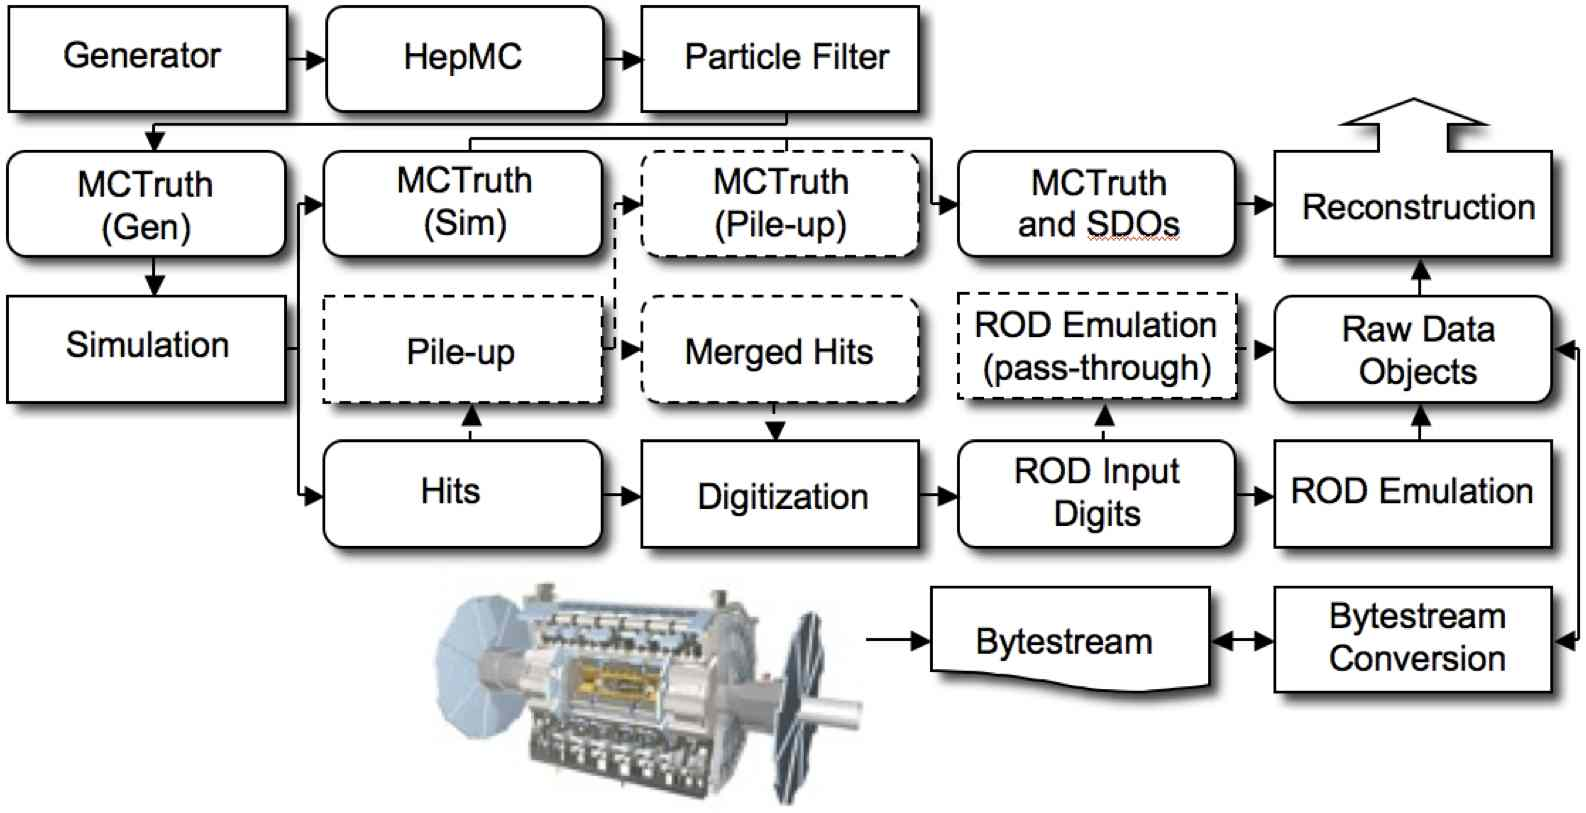
\includegraphics[width=1.0\textwidth]{figures/Simulation/outline_atalsSimulation_v2.png}
  \caption{The flow of the ATLAS simulation software.}
  \label{fig:frame_overview}
\end{figure}

First of all, events are produced by MC generators in standard HepMC format.
The events can be filtered at generation time with some certain requresments and then read into the simulation.
During the simulation, particles are propagated through the full ATLAS detector whose configurations can be set by users via GEANT4 toolkit.
The energies deposited in the sensitive regions of the detector are recorded as \textit{hits}, which contains the total energy deposition,
position, and time, and are written to a simulation hit file.
The files are then sent to digitization jobs, in which Simulated Data Objects (SDOs) are created.
In the meatime, the events in "truth" format are also recorded to contain the history of the interactions from the generator, including incoming and outgoing particles.
SDOs can further make the maps between hits in sensitive portions of the detector and truth information of particles in simulation.


